\documentclass[12pt]{report}
\usepackage{graphicx}
\usepackage{float}
\usepackage{lettrine}
\usepackage{caption}
\usepackage{url}
\usepackage[margin=1in]{geometry}
\usepackage{amsmath}
\usepackage{algorithm}
\usepackage[noend]{algpseudocode}
\usepackage{amssymb}

\newcommand\blfootnote[1]{%
  \begingroup
  \renewcommand\thefootnote{}\footnote{#1}%
  \addtocounter{footnote}{-1}%
  \endgroup
}

\title{Verification of Sequential Elliptic Curve Arithmetic Circuits Using Algebraic Geometry}
\author{Jaden Simon - simonjaden223@gmail.com \\ \and
	   Daniel Humeniuk - d.humeniuk@utah.edu}

	   
\begin{document}

\maketitle

\section{Introduction}

For our term project in ECE 5745, we intend to perform verification of a point-scalar multiplier over an ellitpic curve. The design we are working with relies on  one scalar and one point (two evenly sized $x$ and $y$ coordinates) over three busses and multiplied over an arbitrary elliptical curve using modular arithmetic. The design relies on sequential logic so we will be using some techniques from \cite{Kalla} to traverse the circuit.

We will be studying a 3-bit ECC circuit as a proof of concept. ECC relies on a much larger bit count for security, but for time's sake we are verifying a much smaller circuit. For an $n$-bit ECC circuit, we can perform arithmetic over $\mathbb{F}_{2^n}$, which would be a binary elliptic curve. In software, the field is generally $\mathbb{F}_{p}$ where $p$ is a prime number. Such a field is difficult to work on with hardware, so for this project we will focus exclusively on binary elliptic curves. Note that $n$ is ideally a prime number, otherwise a composite field is formed and mathematical techniques can be used to exploit vulnerabilities in the design. 

Arithmetic over fields of $2^n$ is relatively straightforward. Addition is simply bitwise XOR, multiplication can be done with Mastrovito or Montogomery multipliers, and division is finding the greatest common divisor (GCD). GCD will be computed using the binary GCD algorithm, for which a generic circuit implementation can be found in \ref{fig:gcd}. With these basic functions implemented as circuits, we can first create a point-adder. The point-adder will compute the slope $m$ between two points $(x1, y1), (x2, y2)$, then output a new point using the formulas: $x = m^2 + x1 + x2$ and $y = m(x1 + x) + y1$. Point-scalar multiplication can then naively be done using repeated point addition. If time allows, we will create a more sophisticated circuit using point doubling and attempt to verify that as well. For the point-adder, GCD and galois field multiplication will require using sequential verification techniques. 

\begin{figure}
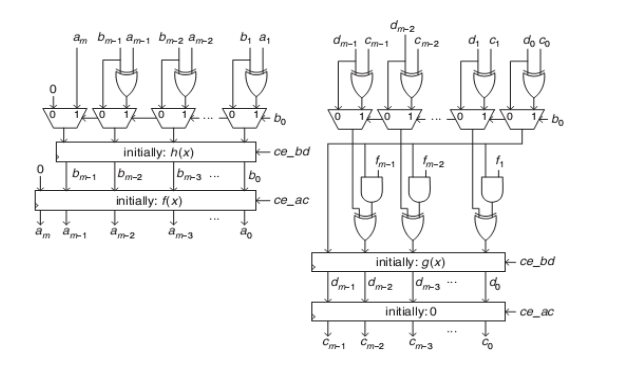
\includegraphics{images/gcd.png}
\caption{Binary GCD Algorithm for $m$ bits \cite{Ajay}}
\label{fig:gcd}
\end{figure}

\section{Our Starting Point}

To begin, we will implement an algebraic geometry based algorithm to implicitly unroll our circuit. The algorithm can be found in \cite{Kalla} and uses projections of varieties to give next state variables in terms of present state variables. Note that our GCD circuit will always terminate after $n^2$ cycles, thus for a 3-bit circuit we will require 9 cycles. Galois field multiplication will always terminate after $n$ cycles. The point multiplier circuit would then require at least $n^3$ cycles to terminate, or 27 iterations. Clearly we can see that as we continue to scale up the ECC circuit, the number of iterations required grows quite rapidly. To verify the large circuits presently used some method of reducing this complexity is required, perhaps by verifying modules individualing then substituting abstractions for full analysis. 

For efficient analysis of circuits, we will need a specific term ordering. The ordering RATO as described in \cite{Kalla} places all bit-level varaibles using a reverse topological order from the circuit first, then word-level next-state outputs, then word-level present-state outputs. The grobner basis can then be computed after adding the vanishing polynomials to the ideal. For our project, we then only need to derive the polynomials from our circuit, then apply RATO, and finally use Singular to compute the grobner basis iteratively. The final grobner basis will contain a polynomial containing only the word-level output with the word-level inputs, which we can then compare to our specification. For the GCD circuit, our spec will just be $R' + A_{init}/B_{init}$ where $R'$ is the next-state result variable, and $A_{init}$, $B_{init}$ are the initial $A$ and $B$ input variables. For the multiplier circuit, our spec is $R' + A_{init}B_{init}$ which \cite{Kalla} already shows the verification of as a proof-of-concept. 

More research will have to be done to define the exact specification for an elliptic curve point adder. Because arithmetic over elliptic curves redefines many of the operations, we cannot just define our specification as one point being added to another. If we define only a single word-level output variable, then our specification will look rather messy as some bits of the output depend only on some bits of the inputs. We may have to define two output word-level variables, one for each coordinate, then apply the above algorithm. This should produce an output resembling the equations from the introduction: $X = ((X2 + Y2)/(X1+Y1))^2 + X1 + X2$ and $Y = ((X2 + Y2)/(X1 + Y1))(X1 + X) + Y1$. Where $X$ and $Y$ are the final next-state result variables and $X1, X2, Y1, Y2$ are the initial input variables. 

A specification polynomial for the point-multiplier seems even more complicated, though it should have a recursive form where the output of the previous point addition feeds into the next point addition. The end result could look quite messy, even for as little as 3 bits which would be up to 8 iterations, or 3 iterations using the more complicated point-doubling method. Further experimentation and research will help us pinpoint what exactly we are looking for when verifying these arithmetic circuits.

\iffalse % Not doing this algorithm 
\begin{algorithm}
\caption{Algebraic Geometry based FSM Traversal}
{\textbf{Input:} The circuit's characteristic polynomial ideal $J_{ckt}$, initial state polynomial $\mathcal{F}(S)$, and LEX term order: bit-level variables $x,s,t >$ PS word S $>$ NS word $T$}
{$from^0=reached=\mathcal{F}(S)$}
{\textbf{Do:}}
\hspace*{6mm}{$i \leftarrow i + 1 $}
\hspace*{6mm}{$G \leftarrow GB(J_{ckt}, J_{v}, from^{i-1}) $}
\hspace*{6mm}{$to^i \leftarrow G \cap \mathbb{F}_{2^k}[T]$}
\hspace*{6mm}{$new^i \leftarrow to^i + (T^{2^k} - T) : reached$}
\hspace*{6mm}{$reached \leftarrow reached*new^i$}
\hspace*{6mm}{$from^i \leftarrow new^i(S$/$T)$}
{\textbf{While:} $new^i != 1$}
{\textbf{Return:} $reached$}

\end{algorithm}

This algorithm will provide us with the the representation of the reached states in every step which we can then over $\mathcal{F}_2^k$. The variables $from$, $reached$, $to$, and $new$ represent the functions of sets in the states.
This algorithm will provide us with the the representation of the reached states in every step which we can then over $\mathbb{F}_{2^k}$. The algorithm uses the Groebner basis of the ideal $J$ and the vanishing ideal $J_0$. This Groebner basis will be used to denote the set of next states in the FSM. 

\fi



\section{Conclusion}
So far we have completed the multiplier and GCD circuits. Our first task will be to apply the sequential circuit verification to the GCD circuit to make sure we understand what is happening and that we can apply the algorithm correctly. Next, we will create the point adder circuit and finalize the specification polynomial. What we find during this step will affect how we verify our full ellitpic curve point multiplier. The final step would of course be verifying the functionality of a full point-scalar multiplier with all internal circuitry exposed. Of course if we have to, we can just replace components of the full circuit with our previously found specifications. This would still be a formal proof of an elliptic curve arithmetic circuit, just not with all internal circuitry exposed. 

\bibliographystyle{IEEEtran}
\bibliography{IEEEabrv,bib/ref}

\end{document}